% Created 2023-07-23 Sun 19:54
% Intended LaTeX compiler: pdflatex
\documentclass[11pt]{article}
\usepackage[utf8]{inputenc}
\usepackage[T1]{fontenc}
\usepackage{graphicx}
\usepackage{longtable}
\usepackage{wrapfig}
\usepackage{rotating}
\usepackage[normalem]{ulem}
\usepackage{amsmath}
\usepackage{amssymb}
\usepackage{capt-of}
\usepackage{hyperref}
\author{holy}
\date{\textit{<2023-07-23 Sun>}}
\title{[emacs] tex install and usage}
\hypersetup{
 pdfauthor={holy},
 pdftitle={[emacs] tex install and usage},
 pdfkeywords={},
 pdfsubject={emacs에서 tex사용},
 pdfcreator={Emacs 30.0.50 (Org mode 9.6.6)}, 
 pdflang={English}}
\begin{document}

\maketitle
\tableofcontents


\section{Local에서의 설치}
\label{sec:org72ad065}
\section{[Local-step1] macTex 설치}
\label{sec:org6434a25}
mac에서는 tex배포판으로 macTex를 다은 받아 설치한다.  \href{https://tug.org/mactex/mactex-download.html}{여기}에서 다운
받는다. mac-tex는 live-tex라는 배포판이 있는데, 거기에 mac관련 요소를
추가해서 만든 배포판이다.
\section{[Local-step2] tex-live update}
\label{sec:org416de3e}
Launchpad에 \TeX{} Live Utility가 있을 것이다. 실행한 후에 패키지
업데이트 다 해준다.
\begin{figure}[htbp]
\centering
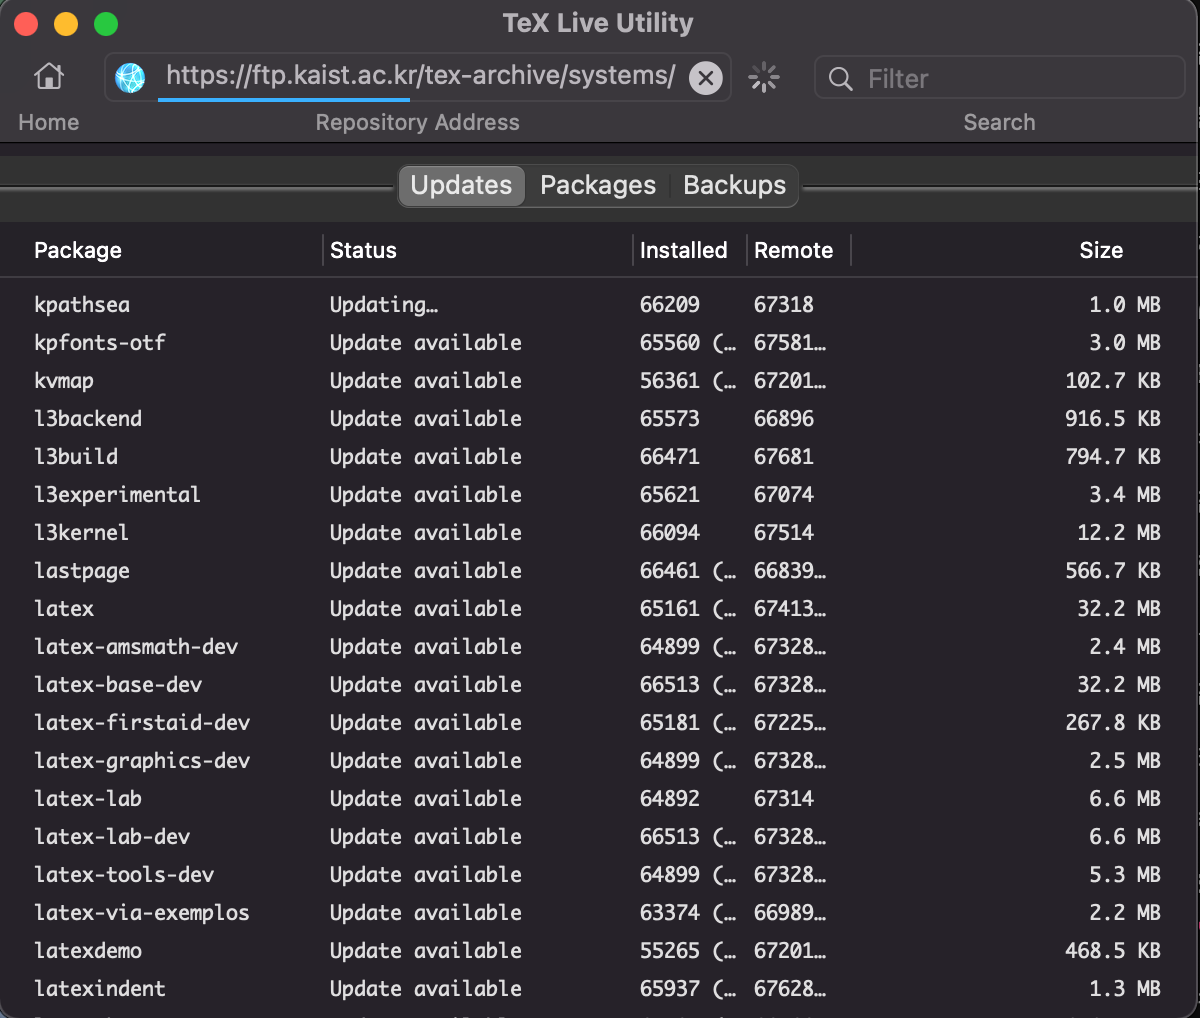
\includegraphics[width=100px]{../static/img/tex/tex-update.png}
\caption{\label{fig:orgd744de5}texlive-update}
\end{figure}
\section{[Local-step3] 사설 repo등록(CTAN and KTUG)}
\label{sec:orga60b3e7}
tlmgr은 brew와 같은 package manager다. brew처럼 저장소에서 package를
가져와서 설치한다. CTAN이 저장소에 해당한다. 영어로된 package는 ctan을
사용하면 되지만, 한글관련해서는 KTUG를 repository로 등록해서
한글폰트같은것을 down받아 사용할려면, KTUG도 등록해서 사용해야 한다.
\href{http://wiki.ktug.org/wiki/wiki.php/KtugPrivateRepository}{여기}를 참조했다.
\subsection{main repo 변경}
\label{sec:org43a56af}
\begin{verbatim}
sudo tlmgr option repository https://mirror.kakao.com/CTAN/systems/texlive/tlnet/
\end{verbatim}
main repo를 kakao서버로 해서 등록했는데, pinning에서 version문제가
있었다. 그래서 아래와 같이 다른 repo로 변경하니 다른 에러가 났다.

\begin{verbatim}
sudo tlmgr option repository http://mirror.ctan.org/systems/texlive/tlnet
\end{verbatim}

그래서 다시 처음의 kakao repo를 다시실행하니 제대로 되었다. 만일 처음 실행한다면,

\subsection{사설 repo(한국)등록}
\label{sec:org9a2b42e}
\begin{verbatim}
sudo tlmgr repository add https://mirror.ischo.org/KTUG/texlive/tlnet ktug
\end{verbatim}
\subsection{pinning추가}
\label{sec:org45a7951}
\begin{verbatim}
sudo tlmgr pinning add ktug "*"
\end{verbatim}
pinning은 ktug라는 사설저장소에서 어떤 package를 tlmgr로
관리할것인지를 정할 수 있게하는 명령어 이다. 여기서 *는 전부 등록해서
관리하겠다는 뜻이다.  그런데 다음과 같은 에러가 난다.

\begin{figure}[htbp]
\centering
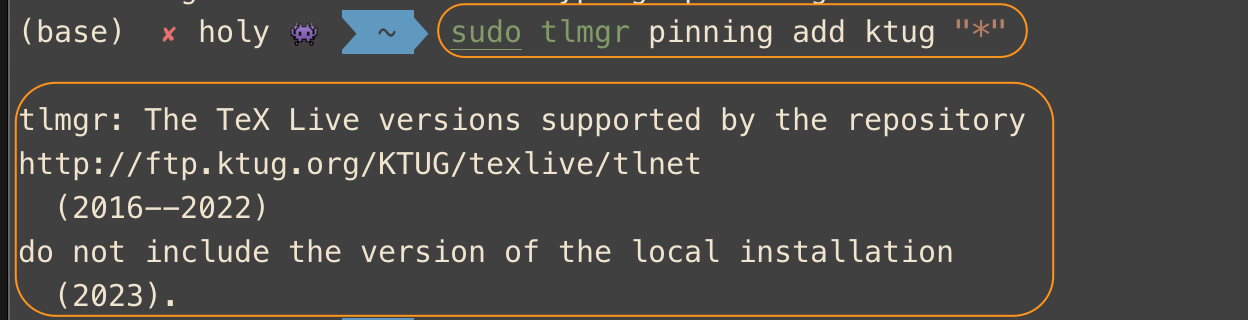
\includegraphics[width=100px]{../static/img/tex/tex-pinning.png}
\caption{\label{fig:org35ee9c5}pinning error}
\end{figure}

이것은 main repo설치와 관련된 문제다. main repo를 제대로 설치하면
문제없이 지나간다.
\section{[Local-step4] 한글 폰트 다운로드 \& 등록}
\label{sec:orga46c395}
step3에서 KTUG라는 사설 repo를 등록한것은 한글 폰트를 다운받기
위함이다.

\begin{verbatim}
sudo tlmgr install nanumttf hcr-lvt
\end{verbatim}
\section{[Local-step5] TexLIVE update}
\label{sec:org735d70d}
이제 전체 package를 update하자.
\begin{verbatim}
sudo tlmgr update --all --self
\end{verbatim}
\section{[Local-step6] XELATEX를 위한 font 설정}
\label{sec:org7fbf0a6}
\href{http://wiki.ktug.org/wiki/wiki.php/\%EC\%84\%A4\%EC\%B9\%98\%ED\%95\%98\%EA\%B8\%B0MacOSX/MacTeX}{여기}에 보면 Mactex를 설치하기의 xelatex설정 부분이 있다. 이것을
따라한다.

참고로 tex는 크게 tex계열과 latex계열이 있다. 두개는 모두 사용법도 다르고
구조도 다르다. 나는 tex문서를 만들고 pdf로 만들려는 목적이기 때문에
XETEX가 아닌 XELATEX를 설치한다. XELATEX가 latex계열이기
때문이다. 

위의 링크에서 Xelatex의 설정이라고 해서 xelatex에 대한 설정인줄
알았는데, 그게 아니라, mac os의 폰트 관리와 Mactex의 폰트관리가 서로
달라서 호환이 안되는 문제가 있다. 이문제를 해결하는 방법을
써놓았다. 아무래도 xelatex를 사용하는데 있어서 한글로 인한 문제가 많이
있어서 그런듯하다.
\subsection{mactex에서 system font찾기.}
\label{sec:org12aa948}
\begin{verbatim}
sudo vi /usr/local/texlive/2023/texmf.cnf
\end{verbatim}
파일을 열고 다음을 추가한다.
\begin{verbatim}
OSFONTDIR = {~/Library/Fonts//;/Library/Fonts//;/System/Library/Fonts//}
\end{verbatim}
보다시피 os의 font가 설치된 directory를 나열한다. mac의 os는 3개의
directory에 저장되어 있기 때문에, mactex가 해당 font-directory에서
font를 찾을 수 있는 경로를 추가해주는 것이다.
\subsection{system에서 mactex font찾기.}
\label{sec:org12be433}
이제 반대로 mac에서도 mactex에 설치된 font를 가져올 수 있어야
한다. 사용자의 \textasciitilde{}/Library/Fonts 아래에 \TeX{} Live의 트루타입과 오픈타입
폴더를 링크해두는 방법이 있다.
\begin{verbatim}
# cd ~/Library/Fonts
ln -s /Library/TeX/Root/texmf-dist/fonts/truetype ~/Library/Fonts/
ln -s /Library/TeX/Root/texmf-dist/fonts/opentype ~/Library/Fonts/
\end{verbatim}
\section{요약}
\label{sec:org8bffa0e}
이렇게 하면, local에서 설치가 끝났다. 그러면 어디서든지 tex파일을
만들고 shell에서 pdflatex를 하면 pdf파일을 만들 수 있다.

\begin{verbatim}
\documentclass{oblivoir},
\begin{document}
\section{헬로우}
안녕하세요, Hello World.
\end{document}
\end{verbatim}

예를 들어서, emacs에서 위와 같이 hello.tex를 만들고, C-c C-c를 누르면
pdf메뉴가 보인다.

\begin{figure}[htbp]
\centering
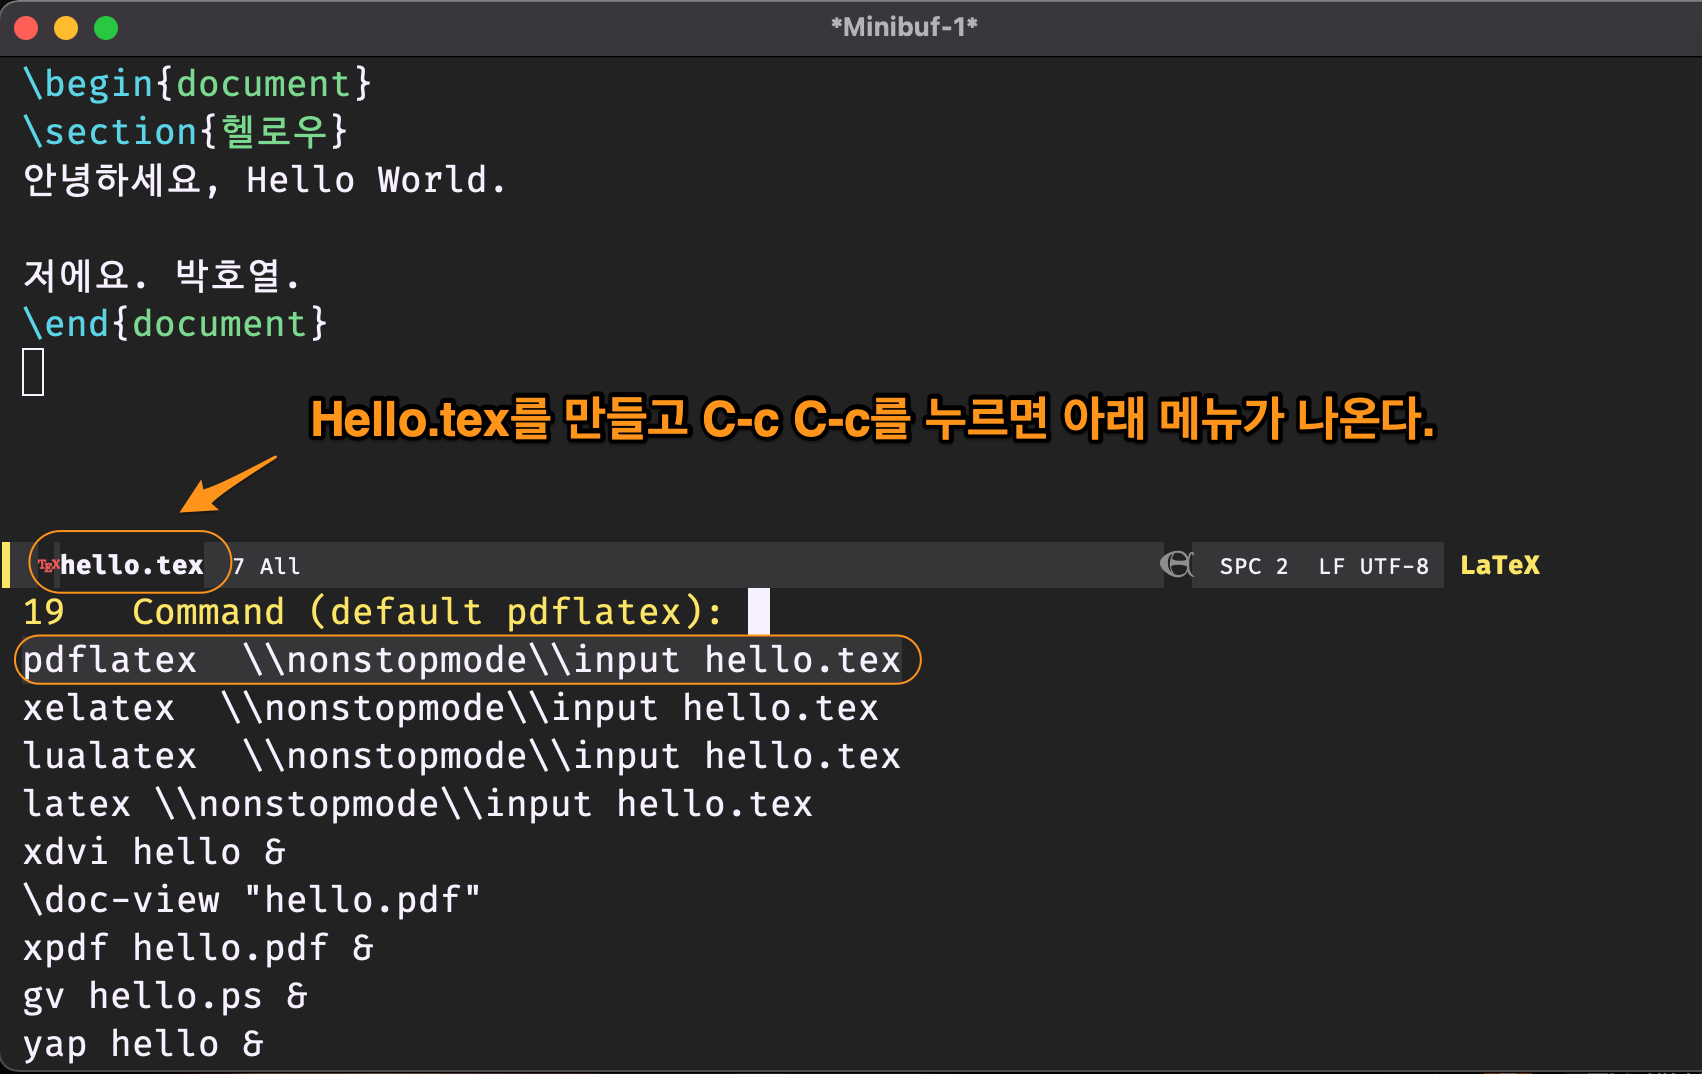
\includegraphics[width=100px]{../static/img/tex/tex1.png}
\caption{\label{fig:orgded014e}tex1}
\end{figure}

근데 pdf파일을 보면 한글이 나오지 않는다. 왜냐면 기본적으로, mactex던
live-tex같은 배포폰은 영문만 지원한다. 위에서 KTUG라는 repo를 등록하고
update했다. 한글폰트도 설치했었다. 한글을 출력할수 있는 package를
깔았다는 얘기다. 다만 사용할 줄을 모르는 것이다. oblivoir라는
한글나오는 documentclass가 있다. 다음과 같이 하면 한글이 나오게 된다.

\begin{verbatim}
\documentclass{oblivoir},
\begin{document}
\section{헬로우}
안녕하세요, Hello World.
\end{document}
\end{verbatim}

한글을 나오게 하는 다른 방법으로 kotex라는 package를 설치하는 방법도
있다. 아래와 같이 하면 된다.

\begin{verbatim}
\usepackage{kotex}  
\begin{document}
\section{헬로우}
안녕하세요, Hello World.
\end{document}
\end{verbatim}

잠깐 한글에 대한 설명을 해야겠다. tex에서 글을 쓰는 방식은 template을
이용해서 문서를 작성한다. 가장 유명한 문서 template은
article이다. 그리고 좀 더 modern한 memoir같은 문서 template이 나오게
된다. 이 template은 모두 영어를 기본으로 한다. 한글이 안
써진다. 위처럼 한글이 pdf로 출력이 되질 않는다. 그런데 ktug라는 곳에서
kotex라는 package를 만들어서, article과 memoir같은 영어권에서만
사용하던 documentclass를 한글에서 사용할 수 있게 했다. 즉,
documentclass를 article로 하고 usepackage\{kotex\}로 하면 한글을 쓸수
있게 했다. 그런데 한글이 조금 부자연스러워서 memoir에 한글을 잘나오게
하는 documentclass를 아예 만들었다. 이게 oblivoir다. 즉 kotex라는
package가 없어도, documentclass\{oblivoir\}를 하면 한글을 사용할 수
있다.
\section{[emacs] 설정.}
\label{sec:org170c6d8}
emacs를 단순히 tex문서를 작성하고 pdf로 뽑아내는데 사용하지
않는다. emacs는 org문서를 pdf로 나타내는데 사용한다.
\end{document}